Our objective this year 
is to generate a video-to-spike train encoder using of-the-shelf components. 
For this, the first approach was to use a biologically plausible functional 
model (Algs. \ref{code-focal-conv} and \ref{code-focal-corr}) that results in images being transformed into rank-ordered spikes~\cite{basab-model}.

\begin{algorithm}[h]
  \caption{FoCal, Part 1}
  \label{code-focal-conv}
  \begin{algorithmic}
    \Procedure{Convolution}{image $I$, kernels $K$}
      \State $C \leftarrow \emptyset$
      \ForAll{$k \in K$}
        \State $C \leftarrow C \cup convolution(k, I)$
      \EndFor
    \EndProcedure
    \algstore{bkbreak}
  \end{algorithmic}
\end{algorithm}
%  \vspace*{-15pt}
\begin{algorithm}[h]
  \caption{FoCal, Part 2}
  \label{code-focal-corr}
  \begin{algorithmic}
    \algrestore{bkbreak}
    \Procedure{Correction}{coeffs $C$, correlations $Q$}
    \State $N \leftarrow \emptyset$ \Comment{Corrected coefficients}
    \Repeat
    \State $m \leftarrow max(C)$
    \State $M \leftarrow M \cup m$
    \State $C \leftarrow C \setminus m$
    \ForAll{$ c \in C$} \Comment{Adjust all remaining c}
    \If{$Q(m, c) \neq 0$} \Comment{Adjust only near}
    \State $c \leftarrow c - m \times Q(m, c)$
    \EndIf
    \EndFor
    \Until{$C = \emptyset$}
    \State \textbf{return} $M$
    \EndProcedure
  \end{algorithmic}
\end{algorithm}

The retina is a thin layer of neural cells located at the back of the eye 
(Fig.~\ref{fig-basic-eye-anatomy}), it is responsible
for the sensing, processing and transmission of visual input~\cite{webvision}. 
At its deepest layer, the retina has a millions of cells known as 
photoreceptors (right of Fig.~\ref{sub-fig-retinal-layers}), they are in charge 
of transforming light into electrical signals. After this step there are three 
layers of neurons that perform different computations such as lateral 
inhibition or centre-surround behaviour (left of 
Fig.~\ref{sub-fig-retinal-layers})~\cite{webvision}. A small area near the 
centre of the retina has very few 
obstacles to obtain light and has the highest resolution, this area is known as the \emph{foveal pit} (small depression on the right of 
Fig.~\ref{sub-fig-eye-schematics}).

\begin{figure}[hbt]
  \centering
  \begin{subfigure}[b]{0.15\textwidth}
    \centering
    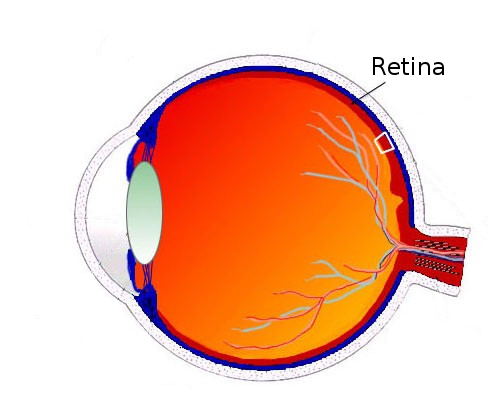
\includegraphics[width=\textwidth,valign=t]{Sagschem}
    \caption{Eye schematics}
    \label{sub-fig-eye-schematics}
  \end{subfigure}
  \begin{subfigure}[b]{0.15\textwidth}
    \centering
    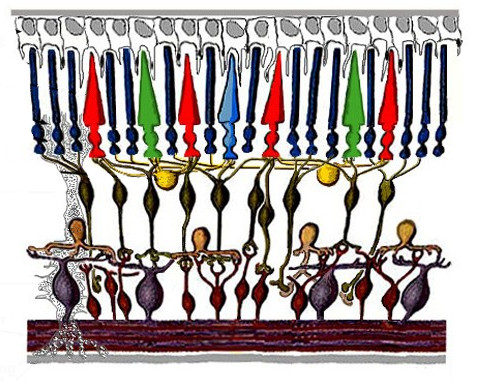
\includegraphics[angle=270,width=\textwidth,valign=t]{schem}
    \caption{Retina}
    \label{sub-fig-retinal-layers}
  \end{subfigure}
  \begin{subfigure}[b]{0.15\textwidth}
    \centering
    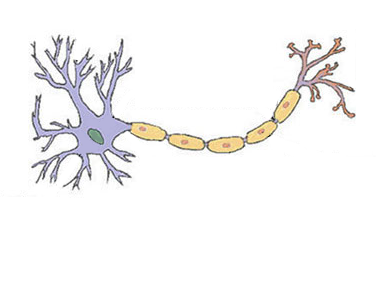
\includegraphics[width=\textwidth,valign=t]{Neuron-___-wikimedia-org}
    \caption{Neuron}
    \label{sub-fig-neuron}
  \end{subfigure}
  
  \caption{Anatomy of the (human) eye \cite{wiki-images}}
  \label{fig-basic-eye-anatomy}
\end{figure}

Algorithms~\ref{code-focal-conv} and \ref{code-focal-corr} model the foveal 
pit. On a first step (Alg.~\ref{code-focal-conv}) we perform a two-dimensional 
\emph{discrete convolution} of the current frame with four \emph{kernels}. 
Each of the ganglion cells are modelled using a Difference of Gaussian 
(Eq.~\ref{eq-dog}) using the parameters shown in 
Table~\ref{tab-kernel-specs}~\cite{field-sensory-coding,basab-model}.
\begin{equation}
\label{eq-dog}
DoG_w(x,y) = \pm\frac{1}{2\pi\sigma_{w,c}^2}e^{\frac{-(x^2 + y^2)}{2\sigma_{w,c}^2}}
\mp\frac{1}{2\pi\sigma_{w,s}^2}e^{\frac{-(x^2 + y^2)}{2\sigma_{w,s}^2}}
\end{equation}
where $\sigma_{w,c}$ and $\sigma_{w,s}$ are the standard deviation for the 
centre and surround components of the DoG at scale $w$ (cell type). The signs 
will be ($-$,$+$) if the ganglion cell is \emph{off-centre} and ($+$,$-$) if it 
is \emph{on-centre}.\\

\begin{figure}[hbt]
  \centering
  \begin{subfigure}[t]{0.15\textwidth}
    \centering
    \captionsetup{justification=centering,margin=0.1cm}
    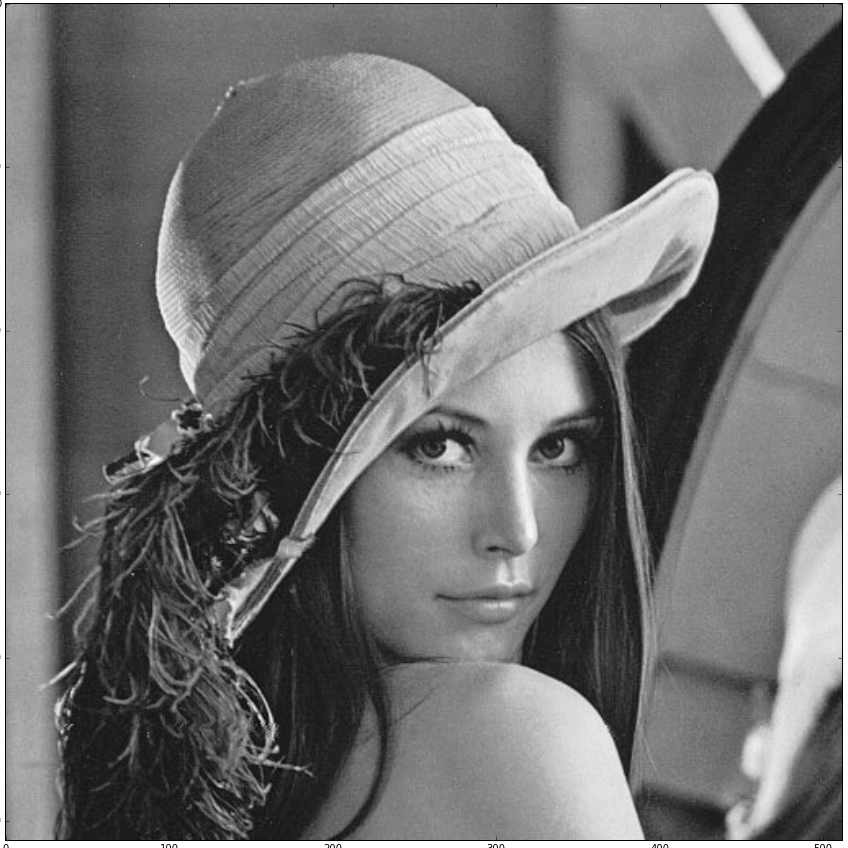
\includegraphics[width=\textwidth]{./Lena-gray}
    \caption{Original image}
    \label{pic-lena}
  \end{subfigure}
  \begin{subfigure}[t]{0.15\textwidth}
    \centering
    \captionsetup{justification=centering,margin=0.1cm}
    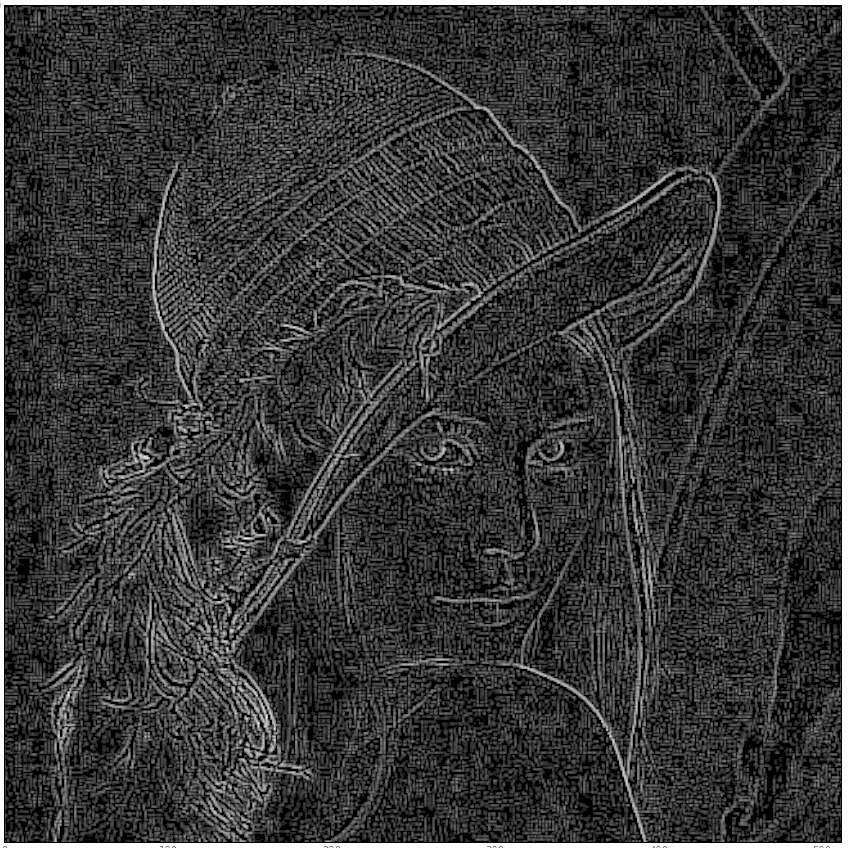
\includegraphics[width=\textwidth]{./Lena-midget_off}
    \caption{Midget OFF-centre}
    \label{pic-lena-M-OFF}
  \end{subfigure}
  \begin{subfigure}[t]{0.15\textwidth}
    \centering
    \captionsetup{justification=centering,margin=0.1cm}
    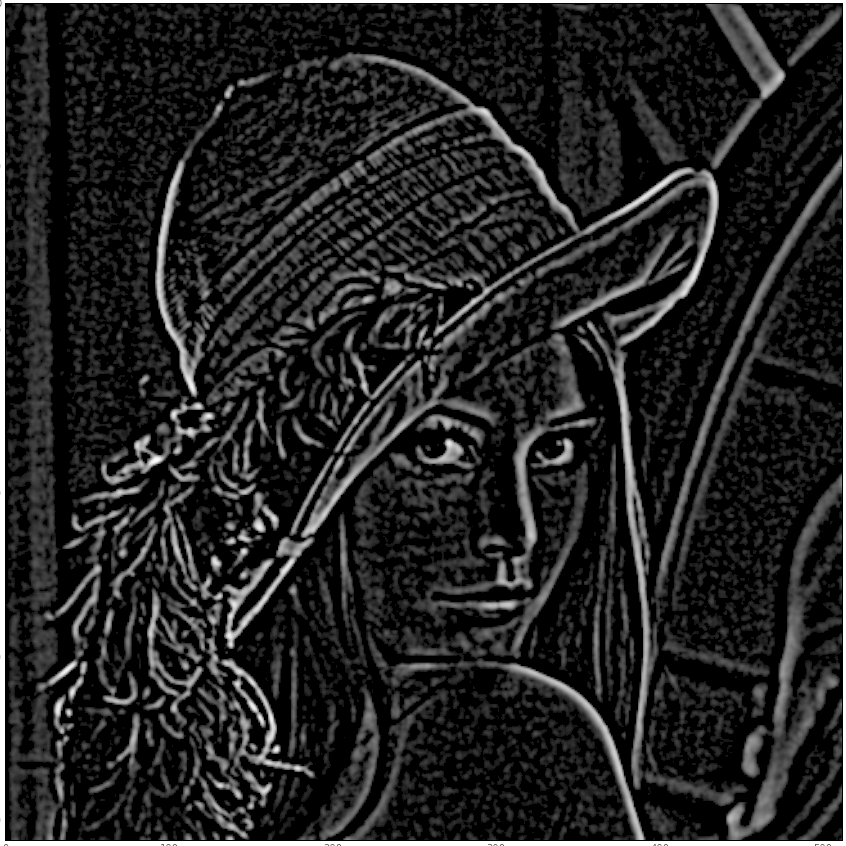
\includegraphics[width=\textwidth]{./Lena-midget_on}
    \caption{Midget ON-centre}
    \label{pic-lena-M-ON}
  \end{subfigure}
  \begin{subfigure}[t]{0.15\textwidth}
    \centering
    \captionsetup{justification=centering,margin=0.1cm}
    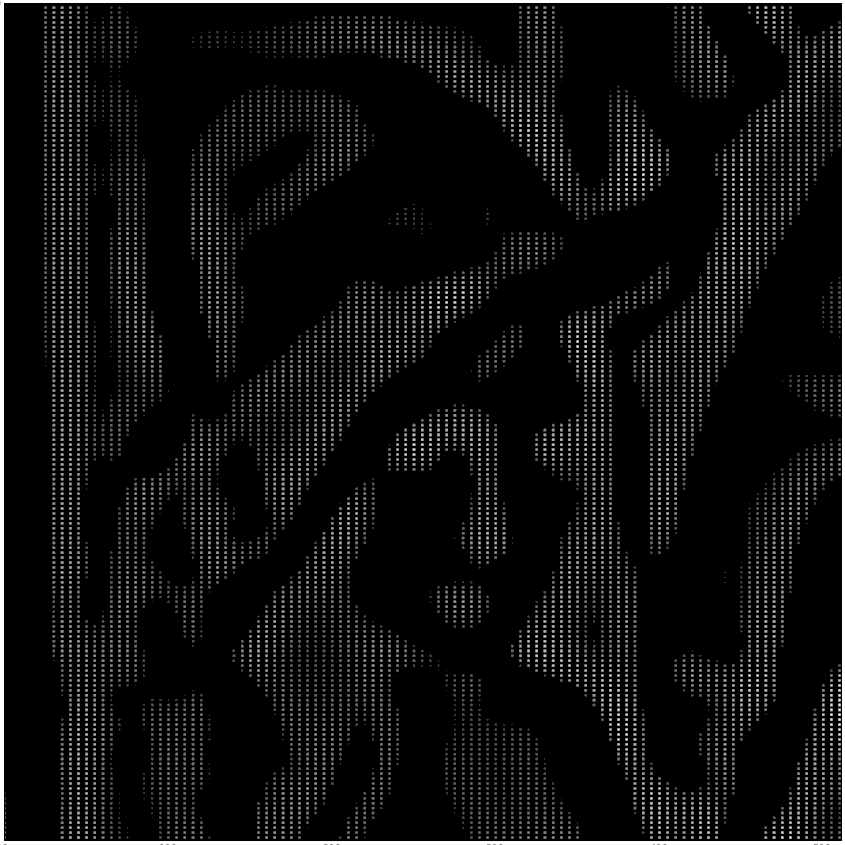
\includegraphics[width=\textwidth]{./Lena-parasol_off}
    \caption{Parasol OFF-centre}
    \label{pic-lena-P-OFF}
  \end{subfigure}
  \begin{subfigure}[t]{0.15\textwidth}
    \centering
    \captionsetup{justification=centering,margin=0.1cm}
    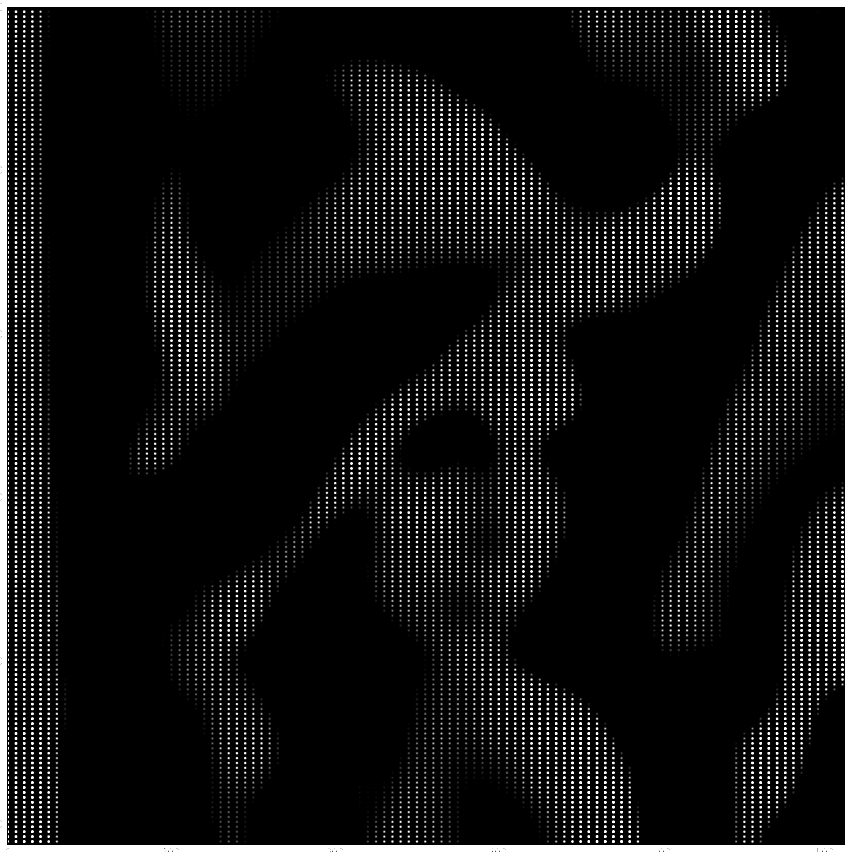
\includegraphics[width=\textwidth]{./Lena-parasol_on}
    \caption{Parasol ON-centre}
    \label{pic-lena-P-ON}
  \end{subfigure}
  \caption{Results of simulating ganglion cells (convolved images are enhanced for better contrast)}
  \label{fig-convolution-results}
\end{figure}
Every pixel in the convolved images (Fig.~\ref{fig-convolution-results}) 
represents a spike emission time, the higher the pixel value, the sooner the 
spike will be sent out.
\begin{table}[htb]
  \caption{Simulation parameters for ganglion cells}
  \centering
%  \begin{TAB}(r,1em,1.5em){|c|c|c|c|c|}{|c|c|c|c|c|} 
  \begin{tabular}{l c c c c}
    \begin{minipage}{1.02cm}Cell type \end{minipage}& 
    \begin{minipage}{0.5cm} \centering Matrix width \end{minipage}&  
    \begin{minipage}{1.3cm}\centering Centre std. dev. ($\sigma_c$)\end{minipage} & 
    \begin{minipage}{1.3cm}\centering Surround std. dev. ($\sigma_s$)\end{minipage} & 
    \begin{minipage}{1.4cm}\centering Sampling resolution (cols, rows)\end{minipage} \\
    \hline
    \begin{minipage}{1.2cm}\vspace*{0.1cm} Midget Off-centre \vspace*{0.005cm} \end{minipage}& 
    \begin{minipage}{0.5cm}\centering$3$ \end{minipage}& 
    $0.8$ & $6.7 \times \sigma_c$ & 1, 1\\
    \begin{minipage}{1.2cm} Midget On-centre \vspace*{0.005cm}\end{minipage} & 
    \begin{minipage}{0.5cm}\centering $11$ \end{minipage}& 
    $1.04$ & $6.7 \times \sigma_c$ &  1, 1\\
    \begin{minipage}{1.2cm}Parasol Off-centre \vspace*{0.005cm}\end{minipage} & 
    \begin{minipage}{1cm}\centering $61$ \end{minipage}& 
    $8$ & $4.8 \times \sigma_c$ & 5, 3 \\
    \begin{minipage}{1.2cm} Parasol On-centre \vspace*{0.005cm}\end{minipage} & 
    \begin{minipage}{0.5cm}\centering $243$\end{minipage} &
    $10.4$ & $4.8 \times \sigma_c$ & 5, 3
  \end{tabular}
  \label{tab-kernel-specs}
  \vspace*{-5pt}
\end{table}
Different ways of performing convolutions on a GPU where implemented, the naïve
does a discrete convolution with the full kernels; for the biggest kernel 
($243\times243$ elements) we were unable to fit it into one of the fast memory
locations of the GPU. We decompose the DoG into two horizontal and two vertical
convolution kernels to perform a separated convolution. This method works best 
on kernels bigger than $3\times3$. The last approach, \emph{Tiled Convolution} 
is reported by Advanced Micro Devices (AMD)~\cite{tiled-convolution}. They only 
present kernels of size $3\times3$, but we have an $11\times11$ convolution 
working; we are still developing solutions for the larger kernels.
Convolution alone is a compute intensive task and we 
obtain about 12 frames-per-second (FPS) on videos with $640\times360$ 8-bit 
grayscale pixel resolution. Encoding was carried out using a desktop computer 
running 64-bit GNU/Linux, with a Core i5-4570 4-core CPU @ 3.20~GHz processor 
with 8~GBytes of 64-bit DDR3 RAM @ 1600~MHz and a GeForce GT 720 GPU with 192 
CUDA cores @ 797~MHz, 1~GBytes of 64-bit DDR3 RAM @ 1800~MHz. %\\

\begin{table}
  \begin{center}
      \caption{Convolution performance comparison.}
      \bgroup
      \def\arraystretch{1.4}
      \begin{tabular}{l c c c c}
        &
        \begin{minipage}{1.2cm}Midget Off-centre\vspace*{0.05cm}\end{minipage} & 
        \begin{minipage}{1.2cm}Midget On-centre\vspace*{0.05cm}\end{minipage}& 
        \begin{minipage}{1.2cm}Parasol Off-centre\vspace*{0.05cm}\end{minipage}& 
        \begin{minipage}{1.2cm}Parasol On-centre\vspace*{0.05cm}\end{minipage}\\
        \hline 
        
        Naïve     & 0.0009s & 0.0031s & 0.0587s & N/A$^{1,2}$ \\ 
        Separated & 0.0021s & 0.0055s & 0.0172s & 0.0472s \\ 
                    % x, y, 0.01756, 0.04500
        Tiled     & 0.0009s & 0.0044s & 0.1643 & N/A$^2$\\
      \end{tabular} 
      \egroup
  {
    \footnotesize 
    \begin{center}
       $^1$ Unable to fit convolution kernel into constant memory.\\
       $^2$ Unable to compile OpenCL code.
    \end{center}
  }
  \end{center}
  \vspace*{-5pt}
\end{table}

In the retina, redundancy of information is reduced via lateral inhibition 
prior to any ganglion cell activity. In this algorithm, we perform a correction 
on the convolved images by adjusting the pixel values
according to the correlation between convolution kernels 
(Alg.~\ref{code-focal-corr}). The results of using correction 
(Fig.~\ref{pic-unfiltered-spikes}) or not (Fig.~\ref{pic-100pc-spikes}) show 
that the convolution stage can only provide redundant information. Furthermore, 
using only 30\% of the corrected weights still provides enough visual 
information to reconstruct the original image~\cite{basab-model}.

\begin{figure}
  \centering
  \begin{subfigure}[t]{0.15\textwidth}
    \centering
    \captionsetup{justification=centering,margin=0.1cm}
    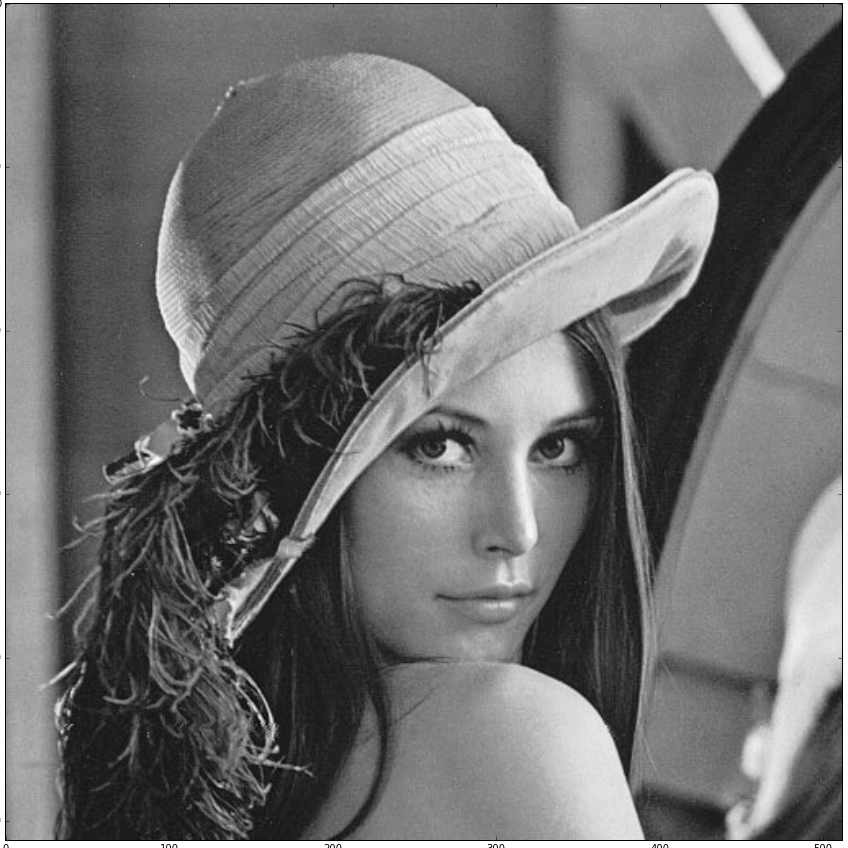
\includegraphics[width=\textwidth]{./Lena-gray}
    \caption{Original image}
    \label{pic-original-lena}
  \end{subfigure}
  \begin{subfigure}[t]{0.15\textwidth}
    \centering
    \captionsetup{justification=centering,margin=0.1cm}
    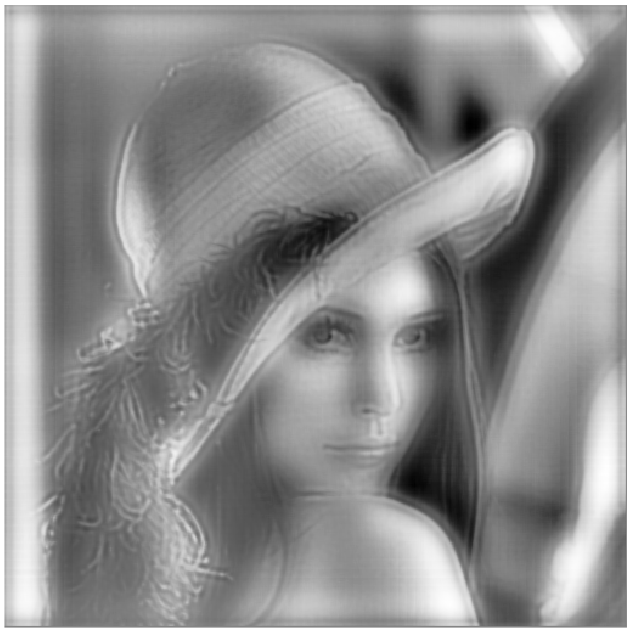
\includegraphics[width=\textwidth]{./final_results-unfiltered}
    \caption{100\% of \\raw spikes}
    \label{pic-unfiltered-spikes}
  \end{subfigure}
  %        \hfill
  \begin{subfigure}[t]{0.15\textwidth}
    \centering
    \captionsetup{justification=centering,margin=0.1cm}
    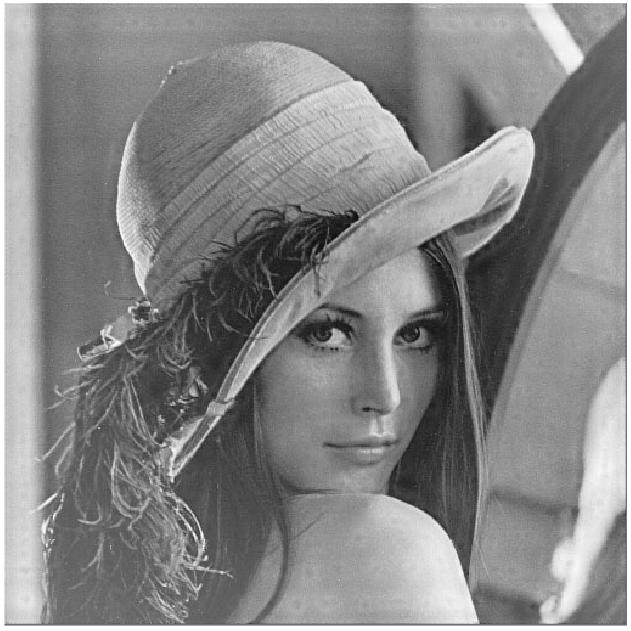
\includegraphics[width=\textwidth]{./final_results-focal-100}
    \caption{100\% of \emph{corrected} spikes}
    \label{pic-100pc-spikes}
  \end{subfigure}
  \caption{Results of reconstruction procedure}
  \label{fig-reconstruction}
  \vspace*{-10pt}
\end{figure}
Correcting the spikes for redundancy is a highly time consuming task which
might be better suited for event-based programming, such as the one found on 
the SpiNNaker platform. We are still working on an implementation for this 
approach.\\

A second way of encoding is to simulate the early stages of the retina, which 
sense changes in intensity on the photoreceptors. This is quite similar to what 
real Dynamic Vision Sensors (DVS) do but with limited dynamic range and lower 
temporal resolution~\cite{aer-retina-bernabe,dvs-zurich}. The main advantage is 
that no specialized hardware is needed and the operation is so fast that any 
recent computer should be able to do it. For this type of encoding procedure we 
hypothesize that the bigger the change, the sooner a cell would spike and, 
thus, we can obtain a spike timings given the difference of two video frames. 
So far we can process about 20 and 25 FPS using a Numpy and an OpenCL back-end, 
respectively (using the same hardware set-up previously described). Although 
it's currently a good approximation, more research on this algorithm is needed 
to better approximate to biology. 
